\section{Introduction}\label{sec:introduction}

\IEEEPARstart{H}{umans} engage naturally in multiple forms of dexterous manipulation that involve grasping, pushing, poking, rolling, and tossing objects \cite{bullock2011classifying}.
Consequently, the development of similar functionality in autonomous machines is an essential milestone for robotics and an area of active research with fundamental work needed ahead \cite{billard2019trends}.
However, the human manipulation skill that has attracted the most attention from roboticists is prehensile manipulation, or \textsl{grasping}.
Manipulation by grasping is attractive primarily because, once an object is grasped, it generally does not need to be tracked over time and uncertainty on its state is reduced. However, grasping is limited in capability by i) reachability of the robot arm, ii) mechanical design limitations of the end-effector, iii) physical properties of the object being manipulated, and iv) accuracy of the perception system.

\textsl{Non-prehensile manipulation} (i.e., any kind of manipulation not involving grasping, hereinafter referred to as NPM) offers a complementary solution to prehensile manipulation by significantly expanding the size (intended as the set of reachable configurations) and dimensionality (intended as the number of degrees of freedom) of the operational space of even the simplest robot manipulator \cite{lynch1999dynamic}.
In other words, NPM can be used to manipulate objects when conventional grasping-based manipulation is infeasible or unnecessary.
Realistic robot applications might expect the robot to operate in dense clutter, in the presence of occlusions, or in ungraspable configurations---for example, the target object is in a pose that is not directly reachable by the end-effector or the target object is too large or too heavy. These applications may result in failure modes for robot operation through traditional grasping. Consequently, in such situations it is beneficial to complement the robot's skillset with NPM primitives. Indeed, NPM can be used both as a skill and a failure recovery mechanism, which points to the versatility of this paradigm.

\begin{figure}
  \centering
    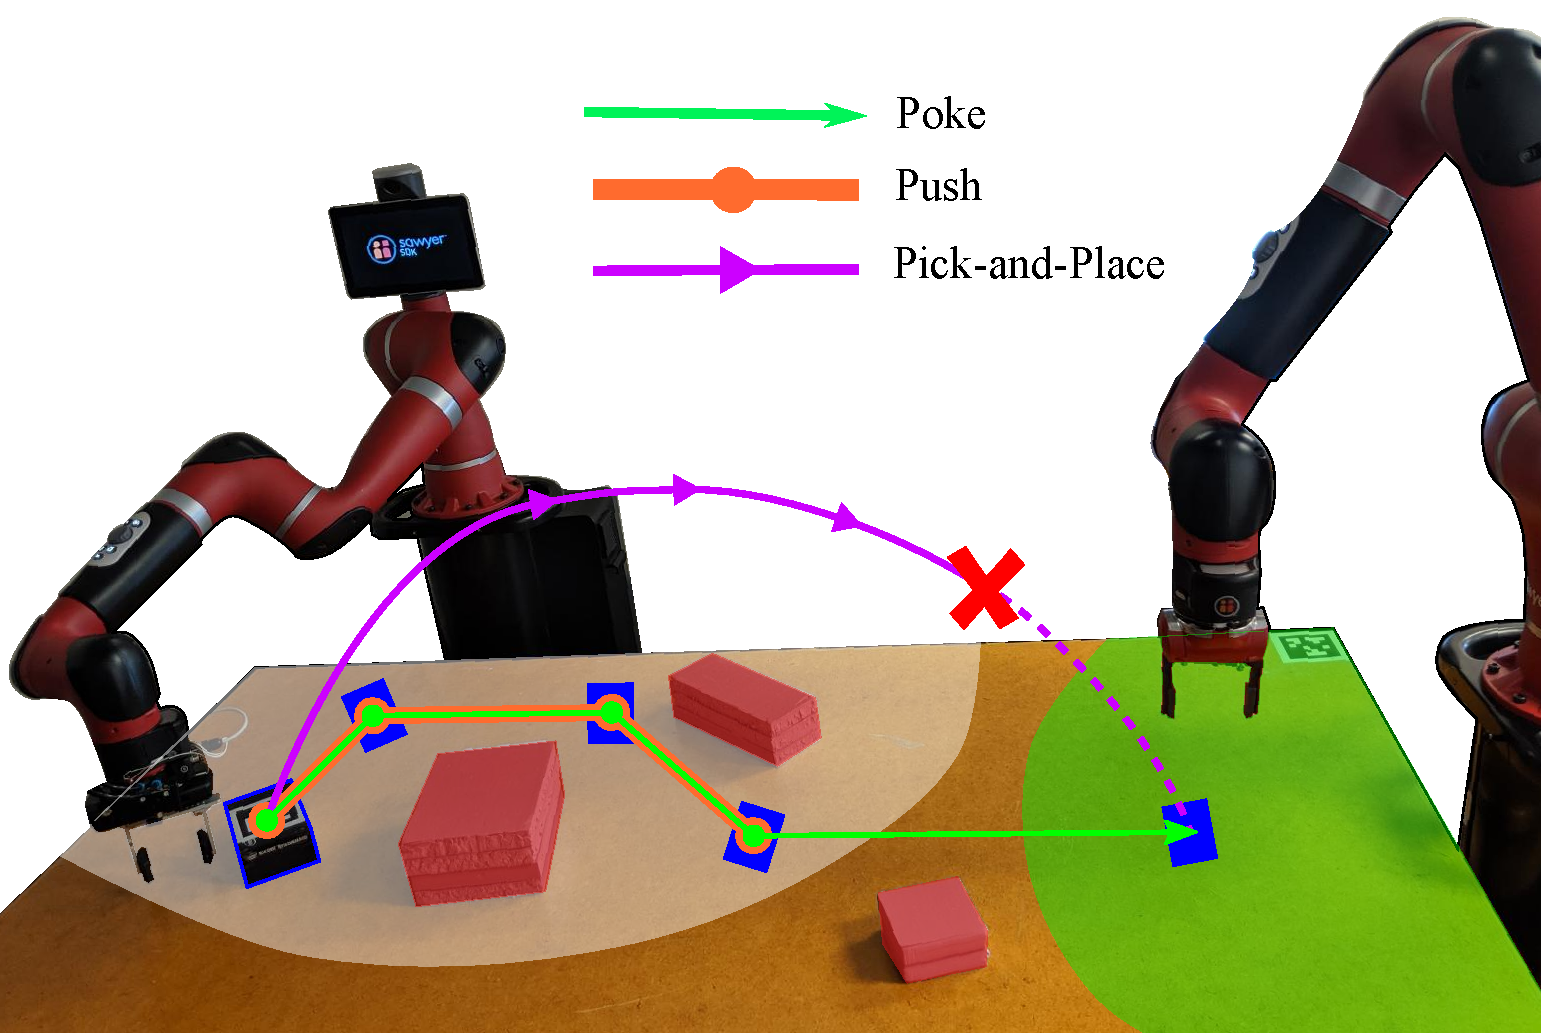
\includegraphics[width=.9\linewidth]{figures/drawing-min.pdf}
  \vspace{-4pt}
  \caption{This work demonstrates poking as a skill and a failure recovery tactic to increase the portfolio of capabilities at the robot's disposal. Here, an object (blue) is located in an obstacle-rich (red) workspace with non-overlapping reachable regions for each robot defined by beige and green shading. The first robot manipulates the object into the green region successfully via poking (path shown in green), but fails to do so via pushing or grasping (paths shown in orange and purple, respectively).\vspace{-14pt}}\label{fig:firstpg}
\end{figure}

In this work, we demonstrate the utility of NPM through poking, a skill that allows fast object manipulation and expands the size of a manipulator's reachable workspace. The basic idea behind this work is detailed in \cref{fig:firstpg}.
\textsl{Poking} is a NPM primitive wherein a robot end-effector applies an instantaneous force to an object of interest to set the object in planar translational and rotational motion (\textsl{impact} phase). The object eventually slows down and comes to rest due to Coulomb friction (\textsl{free-sliding} phase). Poking has a multitude of desirable properties that makes it complementary to grasping and serves as a generalized form of pushing where applied impulse forces are low \cite{Huang-1997-14452, pasricha2021pokerrt}. 
These characteristics make poking especially suitable for industrial settings where robots need to operate in their delineated workspaces alongside other robots or humans while still being able to pass objects. Additionally, in logistics or e-commerce settings, poking can be used for either stowing objects in boxes or in synergy with pick-and-place to optimize operations by increasing speed and coverage area.
In this paper, we design and implement two closed-loop, kinodynamic, sampling-based planners called \textsl{PokeRRT} and \textsl{PokeRRT*} which decouple skill modeling and path planning and specifically focus on leveraging the following advantages of poking over pushing and grasping:
i) it does not require constant contact between the manipulator and the object, therefore greatly expanding the size of the manipulator's workspace,
ii) it does not impose restrictions on the shape or size of objects that can be manipulated, and
iii) it is inherently faster and therefore capable of covering large distances in short periods of time.

After discussing related work (\cref{sec:background}), we present \textsl{PokeRRT} which leverages a simulation engine to generate a collision-free path between two points in the object configuration space (\cref{sec:methods}). We conclude with an experimental validation (\cref{sec:evaluation}) and discussion (\cref{sec:discussion}) of \textsl{PokeRRT} in both simulated and real-world settings.%
